


\begin{frame}
    \frametitle{Cascadia Subduction Zone}
    \begin{figure}
        \includegraphics[width=\textwidth]{JMM/images/meshes/CSZ-lat-lon-4k-with-labels-min.png}
        \caption{\href{https://www.gebco.net/data_and_products/gridded_bathymetry_data/}{GEBCO} bathymetry data of the Cascadia Subduction Zone (CSZ) with ~250m resolution}
    \end{figure}
\end{frame}

\begin{frame}
    \frametitle{Cascadia Subduction Zone}
    \begin{columns}
        \column{0.5\textwidth}
        \includegraphics[width=\textwidth]{JMM/images/intro/ghost-forest.jpeg}
        \column{0.5\textwidth}
        \includegraphics[width=\textwidth]{JMM/images/intro/soil-layers.jpeg}
    \end{columns}
    \caption{Left: Neskowin Ghost Forest; Right: Soil layers in pit (Tofino, BC)}
    \begin{itemize}
        \item Cascadia subduction zone has seen major ruptures in 1700 AD, 1310 AD, 810 AD, 400 AD, 170 BC and 600 BC
        \item Current estimate: 37\% probability of M8.2+ event within 50 years; 10-15\% probability that entire Cascadia subduction zone will rupture with an M9+ event
    \end{itemize}
\end{frame}

\begin{frame}
    \frametitle{Cascadia Subduction Zone Tsunami}
    \movie[width=0.75\textwidth,autostart,loop]{\includegraphics[width=0.75\textwidth]{JMM/images/intro/CSZ_eq.png}}{JMM/images/intro/CSZ_eq.mp4}
    \caption{\href{https://www.youtube.com/watch?v=WuTbDnd_8nA}{Source: Alaska Earthquake Center}}
\end{frame}

\begin{frame}
    \frametitle{Cascadia Subduction Zone Tsunami}
    \movie[width=0.95\textwidth,autostart,loop]{\includegraphics[width=0.95\textwidth]{siam_pp_24/tsunami-clip-75speed.png}}{siam_pp_24/tsunami-clip-75speed.mp4}
    \caption{\href{https://www.youtube.com/watch?v=e5PJQW_6k6M}{Source: Washington State Dept. of Natural Resources}}
\end{frame}

\begin{frame}
    \frametitle{Proposed Sensor Network}
    \begin{figure}
        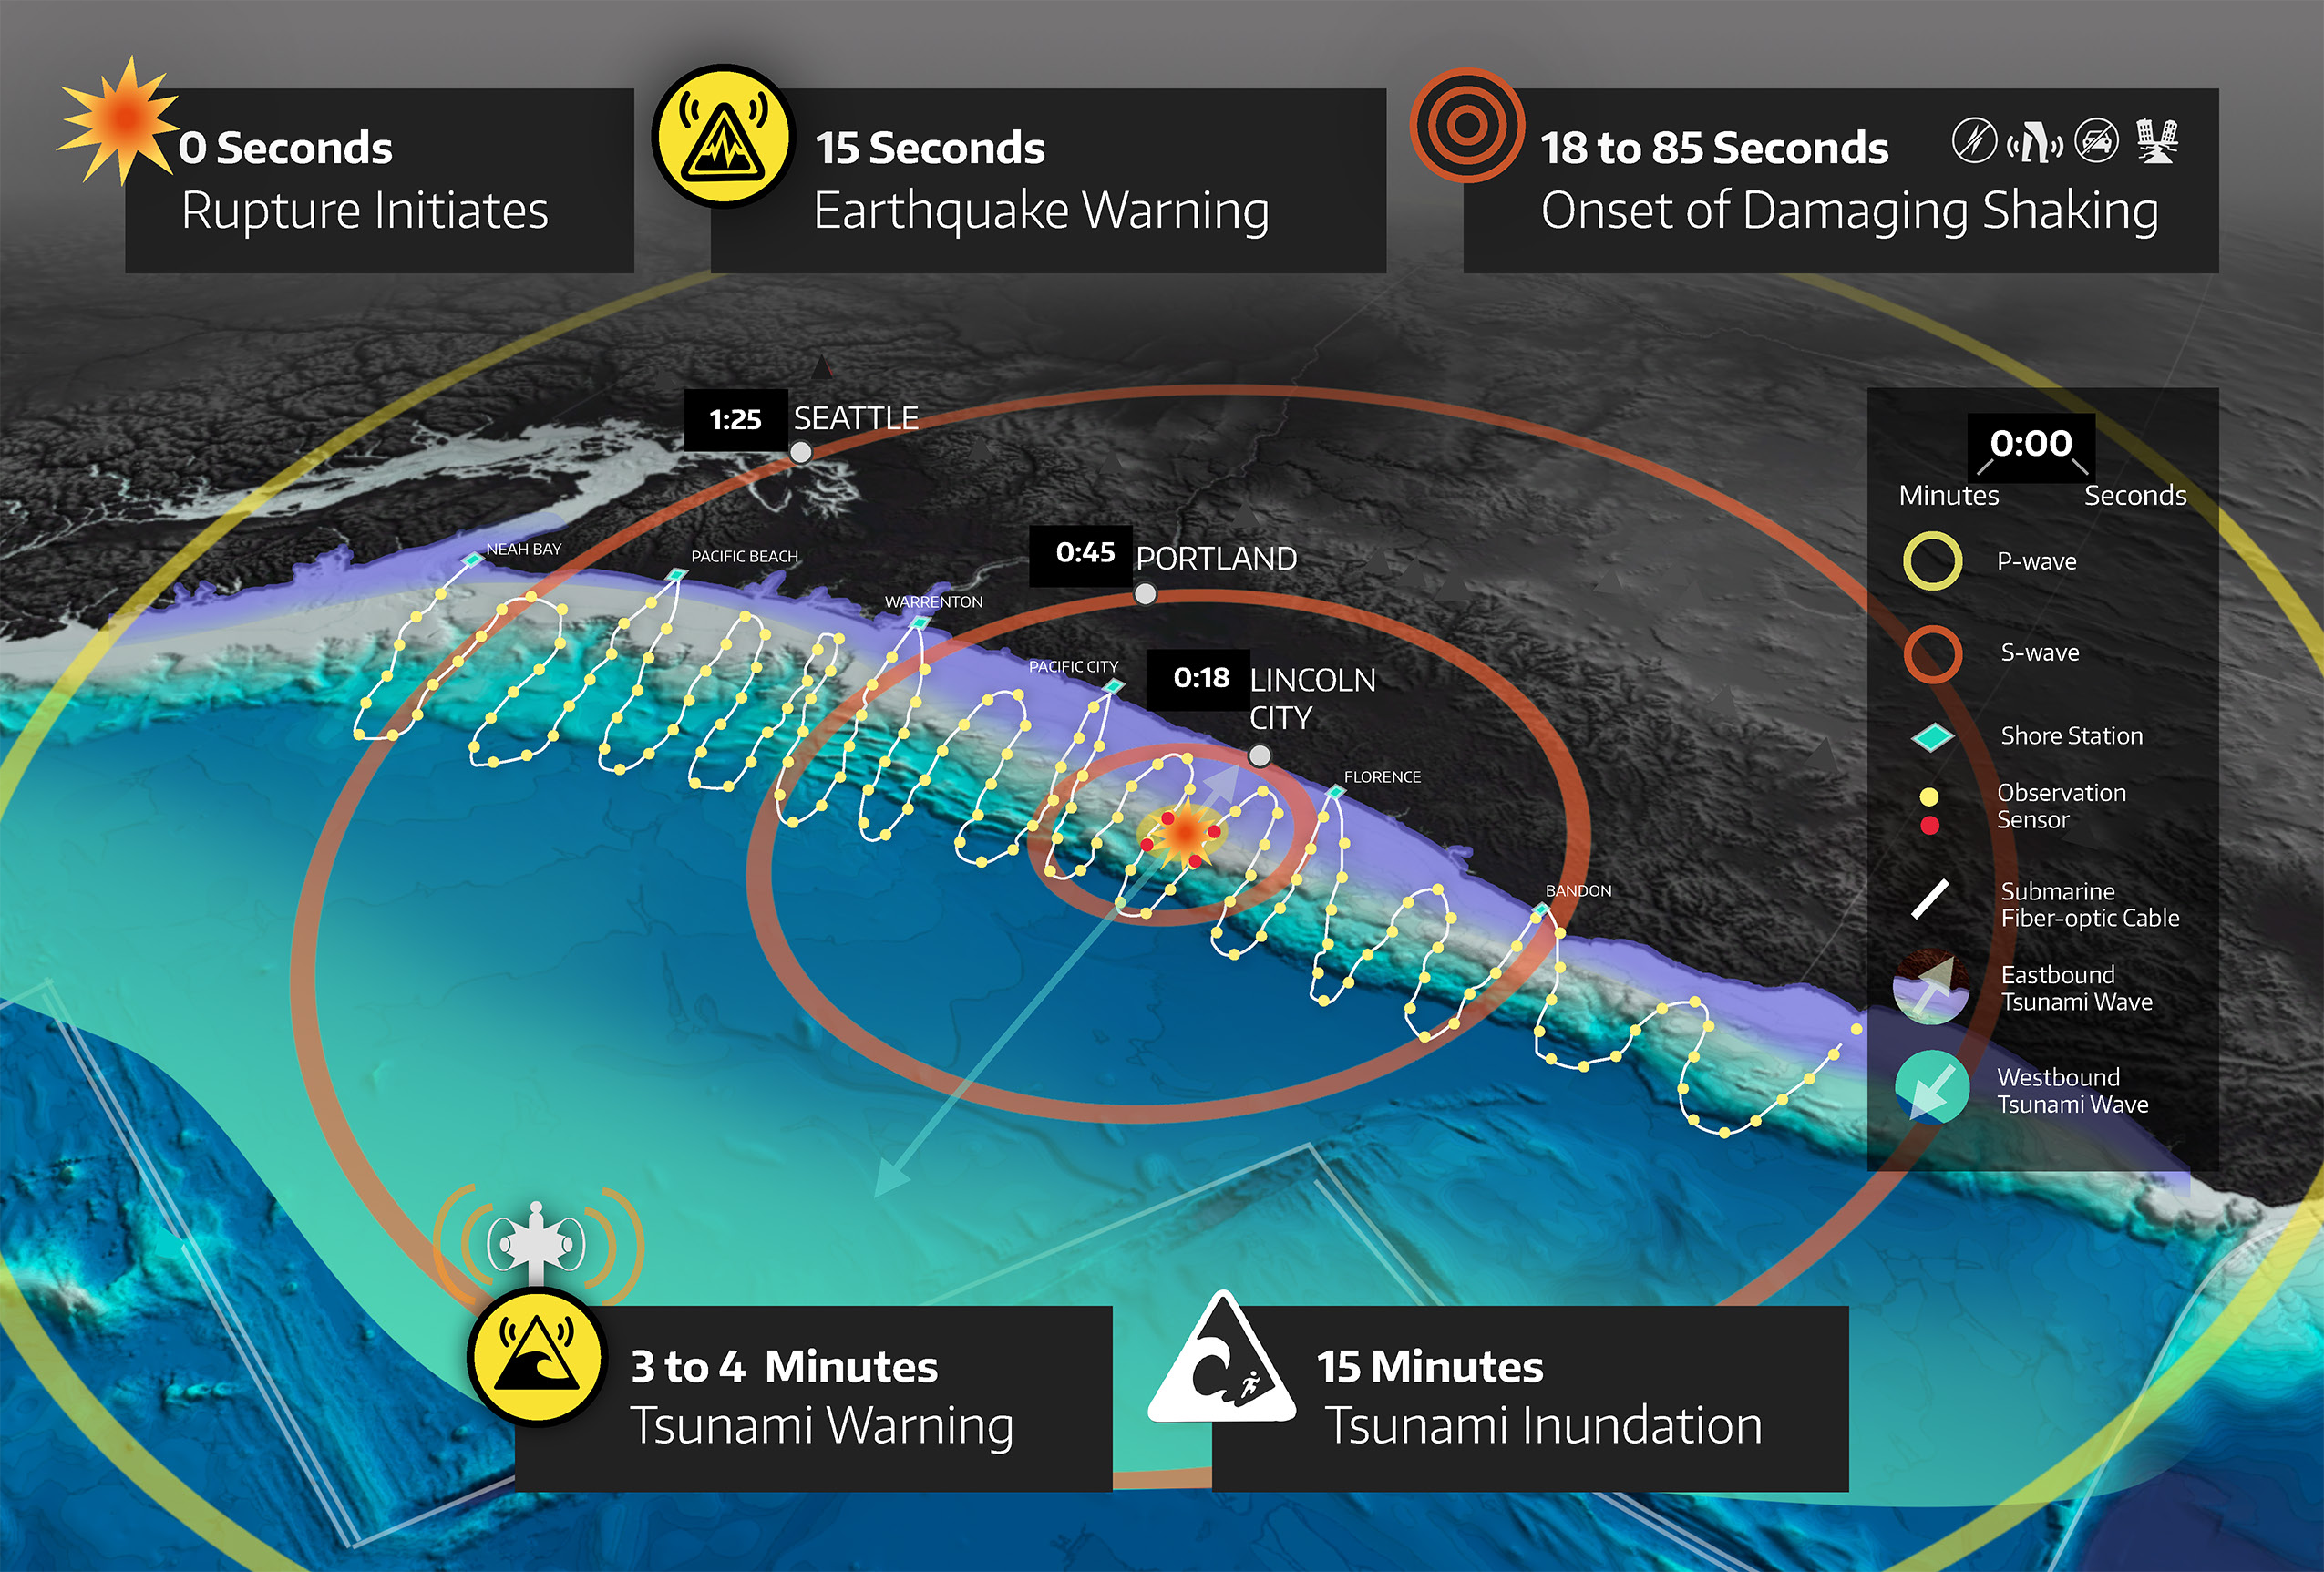
\includegraphics[width=0.75\textwidth]{siam_pp_24/sensor-network.png}
        \caption{\href{http://cascadiaoffshore.org/story/White_Paper.html}{Source: Cascadia Offshore White Paper}}
    \end{figure}
\end{frame}

\begin{frame}
    \frametitle{Cascadia Subduction Zone: Tsunami Early Warning}
    \begin{itemize}
        \item Predict tsunami wave propagation by \textbf{inversion of \underline{near-field} pressure data} recorded during a megathrust rupture
        \item Quantify uncertainty in inverse solution via framework of \textbf{Bayesian inference}
        \item Invert for the spatiotemporal seafloor motion (time-dependent boundary condition) using a (linearized) acoustic-gravity model in the (compressible) deep ocean
        \item Challenges
        \begin{itemize}
            \item Forward problem involves 3D space + time
            \item Parameter is a 2D space + time field
            \item Hyperbolic forward PDEs don't easily lend themselves to surrogates
            \item Inversion computation must be done in \textbf{real time} (i.e. seconds)
        \end{itemize}
    \end{itemize}
\end{frame}

